% Chapter 10: Comprehensive Review
% Harvard-quality academic presentation
% Bachelor program, Bucharest University of Economic Studies

\documentclass[9pt, aspectratio=169, t]{beamer}

% Ensure content fits on slides
\setbeamersize{text margin left=8mm, text margin right=8mm}

%=============================================================================
% THEME AND STYLE CONFIGURATION
%=============================================================================
\usetheme{default}
% Using default theme for clean header/footer control

% Color Palette (matching Redispatch PDF)
\definecolor{MainBlue}{RGB}{26, 58, 110}
\definecolor{AccentBlue}{RGB}{26, 58, 110}
\definecolor{IDAred}{RGB}{205, 0, 0}
\definecolor{DarkGray}{RGB}{51, 51, 51}
\definecolor{MediumGray}{RGB}{128, 128, 128}
\definecolor{LightGray}{RGB}{248, 248, 248}
\definecolor{VeryLightGray}{RGB}{235, 235, 235}
\definecolor{KeynoteGray}{RGB}{218, 218, 218}
\definecolor{SectionGray}{RGB}{120, 120, 120}
\definecolor{FooterGray}{RGB}{100, 100, 100}
\definecolor{Crimson}{RGB}{220, 53, 69}
\definecolor{Forest}{RGB}{46, 125, 50}
\definecolor{Amber}{RGB}{181, 133, 63}
\definecolor{Orange}{RGB}{230, 126, 34}
\definecolor{Purple}{RGB}{142, 68, 173}

% Gradient background (exact Keynote 315° gradient: white to RGB 218,218,218)
\setbeamertemplate{background}{%
    \begin{tikzpicture}[remember picture, overlay]
        \shade[shading=axis, shading angle=315,
        top color=white, bottom color=KeynoteGray]
        (current page.south west) rectangle (current page.north east);
    \end{tikzpicture}%
}
% Fallback solid color for compatibility
\setbeamercolor{background canvas}{bg=}

\setbeamercolor{palette primary}{bg=MainBlue, fg=white}
\setbeamercolor{palette secondary}{bg=MainBlue!85, fg=white}
\setbeamercolor{palette tertiary}{bg=MainBlue!70, fg=white}
\setbeamercolor{structure}{fg=MainBlue}
\setbeamercolor{title}{fg=IDAred}
\setbeamercolor{frametitle}{fg=IDAred, bg=}
\setbeamercolor{block title}{bg=MainBlue, fg=white}
\setbeamercolor{block body}{bg=VeryLightGray, fg=DarkGray}
\setbeamercolor{block title alerted}{bg=Crimson, fg=white}
\setbeamercolor{block body alerted}{bg=Crimson!8, fg=DarkGray}
\setbeamercolor{block title example}{bg=Forest, fg=white}
\setbeamercolor{block body example}{bg=Forest!8, fg=DarkGray}
\setbeamercolor{item}{fg=MainBlue}

% Footer colors (override Madrid theme blue)
\setbeamercolor{author in head/foot}{fg=FooterGray, bg=}
\setbeamercolor{title in head/foot}{fg=FooterGray, bg=}
\setbeamercolor{date in head/foot}{fg=FooterGray, bg=}
\setbeamercolor{section in head/foot}{fg=FooterGray, bg=}
\setbeamercolor{subsection in head/foot}{fg=FooterGray, bg=}

% Bullet styles (apply everywhere including blocks)
\setbeamertemplate{itemize item}{\color{MainBlue}$\boxdot$}
\setbeamertemplate{itemize subitem}{\color{MainBlue}$\blacktriangleright$}
\setbeamertemplate{itemize subsubitem}{\color{MainBlue}\tiny$\bullet$}
\setbeamertemplate{itemize/enumerate body begin}{\normalsize}
\setbeamertemplate{itemize/enumerate subbody begin}{\normalsize}

% Item spacing
\setlength{\leftmargini}{1.5em}
\setlength{\leftmarginii}{1.5em}

\setbeamertemplate{navigation symbols}{}

% TOC with bullets
\setbeamertemplate{section in toc}{\color{MainBlue}$\boxdot$\hspace{0.5em}\inserttocsection}

%=============================================================================
% CUSTOM HEADLINE
%=============================================================================
\setbeamertemplate{headline}{%
    \vskip10pt%
    \hbox to \paperwidth{%
        \hskip0.5cm%
        {\small\color{FooterGray}\renewcommand{\hyperlink}[2]{##2}\insertsectionhead}%
        \hfill%
        \textcolor{FooterGray}{\small\insertframenumber}%
        \hskip0.5cm%
    }%
    \vskip4pt%
    {\color{FooterGray}\hrule height 0.4pt}%
}

%=============================================================================
% CUSTOM FOOTER
%=============================================================================
\usepackage{fontawesome5}

\setbeamertemplate{footline}{%
    {\color{FooterGray}\hrule height 0.4pt}%
    \vskip4pt%
    \hbox to \paperwidth{%
        \hskip0.5cm%
        \textcolor{FooterGray}{\small Time Series Analysis and Forecasting}%
        \hfill%
        \raisebox{-0.1em}{%
            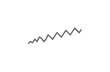
\begin{tikzpicture}[x=0.08em, y=0.08em, line width=0.4pt]
                \draw[FooterGray] (0,3) -- (1,4) -- (2,3.5) -- (3,5) -- (4,4) -- (5,6) -- (6,5.5) -- (7,4) -- (8,5) -- (9,7) -- (10,6) -- (11,5) -- (12,6.5) -- (13,8) -- (14,7) -- (15,6) -- (16,7.5) -- (17,9) -- (18,8) -- (19,7) -- (20,8.5) -- (21,10) -- (22,9) -- (23,8) -- (24,9.5);
            \end{tikzpicture}%
        }%
        \hskip0.5cm%
    }%
    \vskip6pt%
}

%=============================================================================
% PACKAGES
%=============================================================================
\usepackage[utf8]{inputenc}
\usepackage[T1]{fontenc}
\usepackage{amsmath, amssymb, amsthm}
\usepackage{mathtools}
\usepackage{bm}
\usepackage{tikz}
\usetikzlibrary{arrows.meta, positioning, shapes, calc, decorations.pathreplacing, shadings}
\usepackage{booktabs}
\usepackage{multirow}
\usepackage{array}
\usepackage{graphicx}
\usepackage{hyperref}
\usepackage{colortbl}
\hypersetup{colorlinks=true, linkcolor=MainBlue, urlcolor=MainBlue}
\graphicspath{{../logos/}{../charts/}}

%=============================================================================
% QUANTLET COMMAND
%=============================================================================
\newcommand{\quantlet}[2]{%
    \begin{tikzpicture}[remember picture, overlay]
        \node[anchor=south east, inner sep=0pt] at ([xshift=-0.5cm, yshift=0.75cm]current page.south east) {%
            \href{#2}{%
                \raisebox{-0.1em}{\includegraphics[height=0.8em]{ql_logo.png}}%
                \textcolor{MainBlue}{\scriptsize\ #1}%
            }%
        };
    \end{tikzpicture}%
}

%=============================================================================
% CUSTOM TITLE PAGE
%=============================================================================
\defbeamertemplate*{title page}{hybrid}[1][]
{
    \vspace{0.2cm}
    % Logos row - top header (with clickable links)
    \begin{center}\small
        \href{https://www.ase.ro}{\includegraphics[height=0.85cm]{ase_logo.png}}~%
        \href{https://theida.net}{\includegraphics[height=0.85cm]{ida_logo.png}}~%
        \href{https://blockchain-research-center.com}{\includegraphics[height=0.85cm]{brc_logo.png}}~%
        \href{https://www.ai4efin.ase.ro}{\includegraphics[height=0.85cm]{ai4efin_logo.png}}~%
        \href{https://ipe.ro/new}{\includegraphics[height=0.85cm]{acad_logo.png}}~%
        \href{https://www.digital-finance-msca.com}{\includegraphics[height=0.85cm]{msca_logo.png}}%
    \end{center}

    \vspace{0.6cm}

    % Main title with Q logos on sides (with clickable links)
    \begin{center}
        \begin{minipage}{0.1\textwidth}
            \centering
            \href{https://quantlet.com}{\includegraphics[height=1.1cm]{ql_logo.png}}
        \end{minipage}%
        \begin{minipage}{0.78\textwidth}
            \centering
            {\LARGE\bfseries\usebeamercolor[fg]{title}\inserttitle}

            \vspace{0.3cm}

            {\usebeamerfont{subtitle}\usebeamercolor[fg]{title}\insertsubtitle}
        \end{minipage}%
        \begin{minipage}{0.1\textwidth}
            \centering
            \href{https://quantinar.com}{\includegraphics[height=1.1cm]{qr_logo.png}}
        \end{minipage}
    \end{center}

    \vspace{0.6cm}

    % Authors (left aligned)
    \hspace{0.5cm}{\usebeamerfont{author}\insertauthor}

    \vspace{0.3cm}

    % Institute/Affiliations (left aligned)
    \hspace{0.5cm}\begin{minipage}[t]{0.9\textwidth}
        \raggedright\small\insertinstitute
    \end{minipage}
}

%=============================================================================
% THEOREM ENVIRONMENTS
%=============================================================================
\theoremstyle{definition}
\setbeamertemplate{theorems}[numbered]
\newtheorem{defn}{Definition}
\newtheorem{thm}{Theorem}
\newtheorem{prop}{Proposition}
\newtheorem{rmk}{Remark}

%=============================================================================
% CUSTOM COMMANDS
%=============================================================================
\newcommand{\E}{\mathbb{E}}
\newcommand{\Var}{\text{Var}}
\newcommand{\Cov}{\text{Cov}}
\newcommand{\Corr}{\text{Corr}}
\newcommand{\R}{\mathbb{R}}
\newcommand{\N}{\mathbb{N}}
\newcommand{\Z}{\mathbb{Z}}
\newcommand{\B}{\mathbf{B}}
\newcommand{\imark}{\textcolor{MainBlue}{\textbullet}}
\newcommand{\RMSE}{\text{RMSE}}
\newcommand{\MAE}{\text{MAE}}
\newcommand{\MAPE}{\text{MAPE}}

%=============================================================================
% TITLE INFORMATION
%=============================================================================
\title[Time Series Analysis]{Time Series Analysis and Forecasting}
\subtitle{Chapter 10: Comprehensive Review}
\author[D.T. Pele]{Daniel Traian PELE}
\institute{Bucharest University of Economic Studies\\
IDA Institute Digital Assets\\
Blockchain Research Center\\
AI4EFin Artificial Intelligence for Energy Finance\\
Romanian Academy, Institute for Economic Forecasting\\
MSCA Digital Finance}
\date{}

\begin{document}

% Title page (no header/footer)
{
\setbeamertemplate{headline}{}
\setbeamertemplate{footline}{}
\begin{frame}
    \titlepage
\end{frame}
}

%=============================================================================
% TABLE OF CONTENTS
%=============================================================================
\begin{frame}{Outline}
    \tableofcontents
\end{frame}

%=============================================================================
% SECTION 1: METHODOLOGY
%=============================================================================
\section{Forecasting Methodology}

\begin{frame}{The Scientific Approach to Forecasting}
    \begin{block}{Research Question}
        How do we \textbf{rigorously evaluate} forecast performance while avoiding overfitting?
    \end{block}

    \vspace{0.3cm}

    \begin{alertblock}{The Fundamental Problem}
        \begin{itemize}
            \item In-sample fit $\neq$ Out-of-sample performance
            \item Models can ``memorize'' training data without learning patterns
            \item \textbf{Solution}:
                \begin{itemize}
                    \item Proper train/validation/test methodology
                \end{itemize}
            \end{itemize}
    \end{alertblock}

    \vspace{0.3cm}

    \begin{exampleblock}{Key Principle}
        ``The test set must remain \textbf{untouched} until final evaluation.'' \\
        \hfill --- Standard practice in machine learning and econometrics
    \end{exampleblock}
\end{frame}

\begin{frame}{Train/Validation/Test Framework}
    \begin{center}
        \includegraphics[width=0.9\textwidth]{../charts/train_val_test_split.pdf}
    \end{center}

    \begin{columns}[T]
        \column{0.33\textwidth}
        \begin{block}{Training Set}
            \begin{itemize}
                \item Fit parameters
                \item Largest portion
            \end{itemize}
        \end{block}

        \column{0.33\textwidth}
        \begin{block}{Validation Set}
            \begin{itemize}
                \item Compare models
                \item Tune hyperparams
            \end{itemize}
        \end{block}

        \column{0.33\textwidth}
        \begin{block}{Test Set}
            \begin{itemize}
                \item \textbf{Held out}
                \item Final metrics
            \end{itemize}
        \end{block}
    \end{columns}
    \quantlet{TSA\_ch10\_train\_val\_test\_split}{https://github.com/QuantLet/TSA/tree/main/TSA_ch10/TSA_ch10_train_val_test_split}
\end{frame}

\begin{frame}{Evaluation Metrics}
    \begin{defn}[Forecast Error Metrics]
        Let $y_t$ be actual, $\hat{y}_t$ forecast:
        \vspace{-0.2cm}
        \begin{align*}
            \RMSE = \sqrt{\frac{1}{n}\sum_{t}(y_t - \hat{y}_t)^2}, \quad
            \MAE = \frac{1}{n}\sum_{t}|y_t - \hat{y}_t|, \quad
            \MAPE = \frac{100\%}{n}\sum_{t}\left|\frac{y_t - \hat{y}_t}{y_t}\right|
        \end{align*}
    \end{defn}

    \begin{columns}[T]
        \column{0.5\textwidth}
        \begin{exampleblock}{When to Use Each}
            \begin{itemize}
                \item \textbf{RMSE}: Penalizes large errors
                \item \textbf{MAE}: Robust to outliers
                \item \textbf{MAPE}: Scale-independent (\%)
            \end{itemize}
        \end{exampleblock}

        \column{0.5\textwidth}
        \begin{alertblock}{Caution}
            \begin{itemize}
                \item MAPE undefined when $y_t = 0$
                \item Compare on \textbf{same} test set
                \item Report \textbf{out-of-sample} metrics
            \end{itemize}
        \end{alertblock}
    \end{columns}
\end{frame}

%=============================================================================
% SECTION 2: BITCOIN VOLATILITY
%=============================================================================
\section{Case Study 1: Bitcoin Volatility (GARCH)}

\begin{frame}{Bitcoin: Problem Statement}
    \begin{block}{Research Question}
        Can we forecast Bitcoin's \textbf{volatility} using GARCH models?
    \end{block}

    \vspace{0.2cm}

    \begin{columns}[T]
        \column{0.5\textwidth}
        \textbf{Data Characteristics}
        \begin{itemize}
            \item Source: Yahoo Finance (BTC-USD)
            \item Period: Jan 2019 -- Jan 2025
            \item Frequency: Daily
            \item Observations: $\approx 2,200$ days
        \end{itemize}

        \vspace{0.3cm}

        \textbf{Stylized Facts}
        \begin{itemize}
            \item Returns: near-zero mean
            \item Fat tails (kurtosis $> 3$)
            \item Volatility clustering
        \end{itemize}

        \column{0.5\textwidth}
        \begin{alertblock}{Key Insight}
            Financial returns are typically:
            \begin{itemize}
                \item \textbf{Unpredictable} in mean
                \item \textbf{Predictable} in variance
            \end{itemize}

            \vspace{0.2cm}
            $\Rightarrow$ Focus on \textbf{volatility forecasting}
        \end{alertblock}
    \end{columns}
\end{frame}

\begin{frame}{Bitcoin: Volatility Clustering}
    \begin{center}
        \includegraphics[width=0.82\textwidth]{../charts/btc_returns.pdf}
    \end{center}
    \vspace{-0.2cm}
    \begin{exampleblock}{Observation}
        Large returns follow large returns, small follow small---\textbf{volatility clustering}.
    \end{exampleblock}
    \quantlet{TSA\_ch10\_btc\_returns}{https://github.com/QuantLet/TSA/tree/main/TSA_ch10/TSA_ch10_btc_returns}
\end{frame}

\begin{frame}{Bitcoin: Evidence for GARCH}
    \begin{columns}[T]
        \column{0.5\textwidth}
        \begin{center}
            \includegraphics[width=0.95\textwidth]{../charts/btc_squared_returns.pdf}
        \end{center}
        {\footnotesize Squared returns $r_t^2$ proxy for volatility.}

        \column{0.5\textwidth}
        \begin{center}
            \includegraphics[width=0.95\textwidth]{../charts/btc_acf_squared.pdf}
        \end{center}
        {\footnotesize Significant ACF at multiple lags.}
    \end{columns}

    \vspace{0.1cm}

    \begin{alertblock}{Why GARCH?}
        Significant ACF in $r_t^2$ means \textbf{past volatility predicts future volatility}.
    \end{alertblock}
    \quantlet{TSA\_ch10\_btc\_acf\_squared}{https://github.com/QuantLet/TSA/tree/main/TSA_ch10/TSA_ch10_btc_acf_squared}
\end{frame}

\begin{frame}{GARCH Model Specification}
    \begin{defn}[GARCH(p,q) Model]
        Let $r_t$ denote returns. The GARCH(p,q) model:
        \vspace{-0.2cm}
        \begin{align*}
            r_t &= \mu + \varepsilon_t, \quad \varepsilon_t = \sigma_t z_t, \quad z_t \sim N(0,1) \\
            \sigma_t^2 &= \omega + \sum_{i=1}^{q}\alpha_i \varepsilon_{t-i}^2 + \sum_{j=1}^{p}\beta_j \sigma_{t-j}^2
        \end{align*}
        \vspace{-0.3cm}
        where $\omega > 0$, $\alpha_i \geq 0$, $\beta_j \geq 0$, and $\sum \alpha_i + \sum \beta_j < 1$.
    \end{defn}

    \begin{columns}[T]
        \column{0.5\textwidth}
        \begin{block}{Model Variants}
            \begin{itemize}
                \item \textbf{GARCH(1,1)}: Most common
                \item \textbf{GJR-GARCH}: Leverage effect
                \item \textbf{EGARCH}: Asymmetric shocks
            \end{itemize}
        \end{block}

        \column{0.5\textwidth}
        \begin{exampleblock}{Interpretation}
            \begin{itemize}
                \item $\alpha$: Impact of past shocks
                \item $\beta$: Persistence of volatility
                \item $\alpha + \beta \approx 1$: High persistence
            \end{itemize}
        \end{exampleblock}
    \end{columns}
\end{frame}

\begin{frame}{Bitcoin: Data Split and Stationarity}
    \begin{columns}[T]
        \column{0.5\textwidth}
        \begin{block}{Data Split}
            \begin{center}
            \begin{tabular}{lrr}
                \toprule
                \textbf{Set} & \textbf{Period} & \textbf{N} \\
                \midrule
                Training (70\%) & 2019-01 to 2023-03 & 1,543 \\
                Validation (20\%) & 2023-03 to 2024-06 & 441 \\
                Test (10\%) & 2024-06 to 2025-01 & 221 \\
                \midrule
                \textbf{Total} & & \textbf{2,205} \\
                \bottomrule
            \end{tabular}
            \end{center}
        \end{block}

        \column{0.5\textwidth}
        \begin{block}{Stationarity Tests}
            \begin{center}
            \begin{tabular}{lcc}
                \toprule
                \textbf{Series} & \textbf{ADF} & \textbf{Result} \\
                \midrule
                Prices & $p = 0.50$ & Non-stationary \\
                Returns & $p < 0.01$ & \textcolor{Forest}{Stationary} \\
                \bottomrule
            \end{tabular}
            \end{center}

            \vspace{0.3cm}

            $\Rightarrow$ Model \textbf{returns}, not prices
        \end{block}
    \end{columns}

    \vspace{0.3cm}

    \begin{alertblock}{Why Stationarity Matters}
        GARCH requires weakly stationary input. Prices follow random walk; returns are stationary.
    \end{alertblock}
\end{frame}

\begin{frame}{Bitcoin: Model Selection on Validation Set}
    \begin{block}{Methodology}
        Fit each model on \textbf{training data}, evaluate on \textbf{validation set}.
    \end{block}

    \vspace{0.3cm}

    \begin{center}
    \begin{tabular}{lcccl}
        \toprule
        \textbf{Model} & \textbf{AIC} & \textbf{BIC} & \textbf{Val MAE} & \textbf{Selection} \\
        \midrule
        GARCH(1,1) & 6,994.8 & 7,020.6 & \textbf{2.638} & \cellcolor{Forest!20}\textbf{Best} \\
        GARCH(2,1) & 6,993.7 & 7,024.6 & 2.640 & \\
        GJR-GARCH(1,1) & 6,983.7 & 7,014.6 & 2.669 & \\
        EGARCH(1,1) & --- & --- & --- & Failed$^*$ \\
        \bottomrule
    \end{tabular}
    \end{center}

    \vspace{0.1cm}
    {\footnotesize $^*$Analytic forecasts not available for $h > 1$}

    \vspace{0.3cm}

    \begin{exampleblock}{Result}
        \textbf{GARCH(1,1)} selected based on lowest validation MAE for volatility forecasts.
    \end{exampleblock}
\end{frame}

\begin{frame}{Bitcoin: Final Test Set Evaluation}
    \begin{center}
        \includegraphics[width=0.62\textwidth]{../charts/garch_forecast.pdf}
    \end{center}
    \vspace{-0.2cm}
    \begin{columns}[T]
        \column{0.5\textwidth}
        \begin{block}{Parameters}
            $\omega=0.87$, $\alpha=0.09$, $\beta=0.84$\\
            $\alpha + \beta = 0.93$ (high persistence)
        \end{block}

        \column{0.5\textwidth}
        \begin{exampleblock}{Test Performance}
            MAE = 1.82, RMSE = 2.14\\
            Rolling forecasts track volatility well.
        \end{exampleblock}
    \end{columns}
    \quantlet{TSA\_ch10\_garch\_forecast}{https://github.com/QuantLet/TSA/tree/main/TSA_ch10/TSA_ch10_garch_forecast}
\end{frame}

\begin{frame}{GARCH: Multi-Step Forecasts Converge}
    \begin{center}
        \includegraphics[width=0.58\textwidth]{../charts/garch_convergence.pdf}
    \end{center}
    \vspace{-0.2cm}
    \begin{exampleblock}{Key Insight}
        Multi-step forecasts converge to $\bar{\sigma}^2 = \frac{\omega}{1-\alpha-\beta}$. Use rolling forecasts.
    \end{exampleblock}
    \quantlet{TSA\_ch10\_garch\_convergence}{https://github.com/QuantLet/TSA/tree/main/TSA_ch10/TSA_ch10_garch_convergence}
\end{frame}

\begin{frame}{GARCH: Rolling One-Step-Ahead Solution}
    \begin{center}
        \includegraphics[width=0.85\textwidth]{../charts/rolling_vs_multistep.pdf}
    \end{center}

    \begin{columns}[T]
        \column{0.5\textwidth}
        \begin{block}{Multi-Step (Left)}
            Converges to $\bar{\sigma}^2$ \textcolor{Crimson}{(flat)}
        \end{block}

        \column{0.5\textwidth}
        \begin{exampleblock}{Rolling 1-Step (Right)}
            Re-estimate at each $t$ \textcolor{Forest}{(dynamic)}
        \end{exampleblock}
    \end{columns}
    \quantlet{TSA\_ch10\_rolling\_vs\_multistep}{https://github.com/QuantLet/TSA/tree/main/TSA_ch10/TSA_ch10_rolling_vs_multistep}
\end{frame}

% Removed duplicate slide - content merged into "Bitcoin: Final Test Set Evaluation"

\begin{frame}{Bitcoin: Key Findings}
    \begin{columns}[T]
        \column{0.6\textwidth}
        \begin{block}{Summary}
            \begin{enumerate}
                \item \textbf{Returns are stationary}; prices are not
                \item \textbf{GARCH(1,1)} outperforms more complex variants
                \item \textbf{High persistence} ($\alpha + \beta = 0.93$)
                \item Volatility is \textbf{predictable} even when returns are not
            \end{enumerate}
        \end{block}

        \vspace{0.3cm}

        \begin{exampleblock}{Practical Implications}
            \begin{itemize}
                \item Risk management: VaR, Expected Shortfall
                \item Option pricing requires volatility forecasts
                \item Portfolio optimization with time-varying risk
            \end{itemize}
        \end{exampleblock}

        \column{0.4\textwidth}
        \begin{alertblock}{Limitations}
            \begin{itemize}
                \item GARCH assumes \textbf{symmetric} shocks
                \item Does not capture \textbf{jumps}
                \item Normal distribution may be restrictive
            \end{itemize}
        \end{alertblock}

        \vspace{0.3cm}

        \begin{block}{Extensions}
            \begin{itemize}
                \item Student-t innovations
                \item Realized volatility
                \item HAR models
            \end{itemize}
        \end{block}
    \end{columns}
\end{frame}

%=============================================================================
% SECTION 3: SUNSPOTS
%=============================================================================
\section{Case Study 2: Sunspot Cycles (Fourier)}

\begin{frame}{Sunspots: The 11-Year Solar Cycle}
    \begin{columns}[T]
        \column{0.55\textwidth}
        \begin{center}
            \includegraphics[width=0.95\textwidth]{../charts/sunspots.pdf}
        \end{center}
        {\footnotesize Cycle peaks every 11 years.}

        \column{0.45\textwidth}
        \begin{center}
            \includegraphics[width=0.95\textwidth]{../charts/sunspots_acf.pdf}
        \end{center}
        {\footnotesize ACF peaks at lag 11, 22.}
    \end{columns}

    \vspace{0.1cm}

    \begin{alertblock}{Challenge}
        SARIMA$_{11}$ requires too many parameters. \textbf{Solution}: Use Fourier terms.
    \end{alertblock}
    \quantlet{TSA\_ch10\_sunspots\_acf}{https://github.com/QuantLet/TSA/tree/main/TSA_ch10/TSA_ch10_sunspots_acf}
\end{frame}

\begin{frame}{Fourier Terms for Seasonality}
    \begin{center}
        \includegraphics[width=0.78\textwidth]{../charts/fourier_terms.pdf}
    \end{center}
    \vspace{-0.2cm}
    \begin{columns}[T]
        \column{0.55\textwidth}
        \begin{block}{How It Works}
            $S_t = \sum_{k=1}^{K}\left[\alpha_k \sin\left(\frac{2\pi k t}{s}\right) + \beta_k \cos\left(\frac{2\pi k t}{s}\right)\right]$
        \end{block}

        \column{0.45\textwidth}
        \begin{exampleblock}{Key Insight}
            \begin{itemize}
                \item $K=1$: 2 params
                \item $K=3$: 6 params
            \end{itemize}
        \end{exampleblock}
    \end{columns}
    \quantlet{TSA\_ch10\_fourier\_terms}{https://github.com/QuantLet/TSA/tree/main/TSA_ch10/TSA_ch10_fourier_terms}
\end{frame}

\begin{frame}{Sunspots: Model Selection}
    \begin{block}{Methodology}
        Compare $K = 1, 2, 3, 4$ Fourier harmonics on validation set.
    \end{block}

    \vspace{0.2cm}

    \begin{columns}[T]
        \column{0.5\textwidth}
        \begin{center}
        \textbf{Data Split}
        \begin{tabular}{lrr}
            \toprule
            \textbf{Set} & \textbf{Period} & \textbf{N} \\
            \midrule
            Training (70\%) & 1900--1975 & 76 \\
            Validation (20\%) & 1976--1997 & 22 \\
            Test (10\%) & 1998--2008 & 11 \\
            \midrule
            \textbf{Total} & & \textbf{109} \\
            \bottomrule
        \end{tabular}
        \end{center}

        \column{0.5\textwidth}
        \begin{center}
        \textbf{Model Comparison}
        \begin{tabular}{cccc}
            \toprule
            \textbf{K} & \textbf{AIC} & \textbf{Val RMSE} & \\
            \midrule
            1 & 665.9 & 87.15 & \\
            2 & 668.0 & 86.92 & \\
            \rowcolor{Forest!20} 3 & 671.8 & \textbf{86.81} & Best \\
            4 & 674.5 & 87.93 & \\
            \bottomrule
        \end{tabular}
        \end{center}
    \end{columns}

    \vspace{0.3cm}

    \begin{exampleblock}{Result}
        \textbf{K = 3} Fourier harmonics selected (6 parameters for 11-year cycle).
    \end{exampleblock}
\end{frame}

\begin{frame}{Sunspots: Forecast Results}
    \begin{center}
        \includegraphics[width=0.68\textwidth]{../charts/sunspot_forecast.pdf}
    \end{center}
    \vspace{-0.2cm}
    \begin{columns}[T]
        \column{0.5\textwidth}
        \begin{block}{Model}
            ARIMA(2,0,1) + 3 Fourier terms.
        \end{block}

        \column{0.5\textwidth}
        \begin{exampleblock}{Test Performance}
            RMSE = 31.10, MAE = 25.83.
        \end{exampleblock}
    \end{columns}
    \quantlet{TSA\_ch10\_sunspot\_forecast}{https://github.com/QuantLet/TSA/tree/main/TSA_ch10/TSA_ch10_sunspot_forecast}
\end{frame}

\begin{frame}{Sunspots: Key Takeaways}
    \begin{columns}[T]
        \column{0.5\textwidth}
        \begin{block}{When to Use Fourier Terms}
            \begin{itemize}
                \item Seasonal period $s$ is \textbf{long} (e.g., 11 years, 52 weeks)
                \item SARIMA would require too many seasonal lags
                \item Pattern is \textbf{smooth and periodic}
                \item Multiple cycles need to be captured
            \end{itemize}
        \end{block}

        \vspace{0.2cm}

        \begin{alertblock}{Choosing K}
            Start with $K=1$, increase until validation error stops improving. Too high $K$ = overfitting.
        \end{alertblock}

        \column{0.5\textwidth}
        \begin{exampleblock}{Fourier vs SARIMA}
            \begin{center}
            \begin{tabular}{lcc}
                \toprule
                & \textbf{Fourier} & \textbf{SARIMA} \\
                \midrule
                Long seasons & \checkmark & $\times$ \\
                Short seasons & OK & \checkmark \\
                Parameters & $2K$ & Many \\
                Flexibility & Fixed & Adaptive \\
                \bottomrule
            \end{tabular}
            \end{center}
        \end{exampleblock}

        \vspace{0.2cm}

        \begin{block}{Applications}
            Climate cycles, business cycles, astronomical phenomena
        \end{block}
    \end{columns}
\end{frame}

%=============================================================================
% SECTION 4: UNEMPLOYMENT
%=============================================================================
\section{Case Study 3: Unemployment (Prophet)}

\begin{frame}{Unemployment: Train / Validation / Test Split}
    \begin{center}
        \includegraphics[width=0.78\textwidth]{../charts/unemployment_train_val_test.pdf}
    \end{center}
    \vspace{-0.2cm}
    \begin{block}{Methodology}
        \textbf{Training}: Fit models. \textbf{Validation}: Select best. \textbf{Test}: Final evaluation.
    \end{block}
    \quantlet{TSA\_ch10\_unemployment\_train\_val\_test}{https://github.com/QuantLet/TSA/tree/main/TSA_ch10/TSA_ch10_unemployment_train_val_test}
\end{frame}

\begin{frame}{Unemployment: Preliminary Analysis}
    \begin{center}
        \includegraphics[width=0.75\textwidth]{../charts/unemployment_acf_pacf.pdf}
    \end{center}
    \vspace{-0.2cm}
    \begin{columns}[T]
        \column{0.5\textwidth}
        \begin{block}{ACF Interpretation}
            Slow decay $\Rightarrow$ non-stationary.
        \end{block}

        \column{0.5\textwidth}
        \begin{exampleblock}{PACF Interpretation}
            Spike at lag 1 $\Rightarrow$ AR(1) component.
        \end{exampleblock}
    \end{columns}
    \quantlet{TSA\_ch10\_unemployment\_acf\_pacf}{https://github.com/QuantLet/TSA/tree/main/TSA_ch10/TSA_ch10_unemployment_acf_pacf}
\end{frame}

\begin{frame}{Unemployment: Stationarity Tests}
    \begin{center}
        \includegraphics[height=0.55\textheight, keepaspectratio]{../charts/unemployment_stationarity.pdf}
    \end{center}
    \vspace{-0.2cm}
    \begin{columns}[T]
        \column{0.5\textwidth}
        \begin{alertblock}{Original: ADF p = 0.056}
            Non-stationary (slow ACF decay)
        \end{alertblock}

        \column{0.5\textwidth}
        \begin{exampleblock}{Differenced: ADF p $<$ 0.001}
            Stationary $\Rightarrow$ use $d=1$
        \end{exampleblock}
    \end{columns}
    \quantlet{TSA\_ch10\_unemployment\_stationarity}{https://github.com/QuantLet/TSA/tree/main/TSA_ch10/TSA_ch10_unemployment_stationarity}
\end{frame}

\begin{frame}{Unemployment: Model Selection (Validation Set)}
    \begin{center}
        \includegraphics[width=0.70\textwidth]{../charts/sarima_model_selection.pdf}
    \end{center}
    \vspace{-0.3cm}
    \begin{block}{Best: SARIMA(1,1,1)(1,0,0)$_{12}$}
        Selected by lowest validation RMSE.
    \end{block}
    \quantlet{TSA\_ch10\_sarima\_model\_selection}{https://github.com/QuantLet/TSA/tree/main/TSA_ch10/TSA_ch10_sarima_model_selection}
\end{frame}

\begin{frame}{Unemployment: SARIMA Parameters}
    \begin{center}
        \includegraphics[width=0.65\textwidth]{../charts/sarima_parameters.pdf}
    \end{center}

    \begin{block}{SARIMA(1,1,1)(1,0,0)$_{12}$ fitted on Train+Val (2010-2019)}
        AR(1): $\phi_1 = -0.86$, MA(1): $\theta_1 = 0.78$, SAR(12): $\Phi_1 = -0.08$ (n.s.)
    \end{block}
    \quantlet{TSA\_ch10\_sarima\_parameters}{https://github.com/QuantLet/TSA/tree/main/TSA_ch10/TSA_ch10_sarima_parameters}
\end{frame}

\begin{frame}{Unemployment: SARIMA Diagnostics}
    \begin{center}
        \includegraphics[width=0.40\textwidth]{../charts/sarima_diagnostics.pdf}
    \end{center}
    \vspace{-0.3cm}
    \begin{columns}[T]
        \column{0.5\textwidth}
        \begin{block}{Residuals}
            Histogram, ACF, Q-Q plot.
        \end{block}

        \column{0.5\textwidth}
        \begin{exampleblock}{Ljung-Box p = 0.66}
            No autocorrelation.
        \end{exampleblock}
    \end{columns}
    \quantlet{TSA\_ch10\_sarima\_diagnostics}{https://github.com/QuantLet/TSA/tree/main/TSA_ch10/TSA_ch10_sarima_diagnostics}
\end{frame}

\begin{frame}{Unemployment: SARIMA Rolling Forecast}
    \begin{center}
        \includegraphics[height=0.55\textheight, keepaspectratio]{../charts/sarima_forecast.pdf}
    \end{center}
    \vspace{-0.3cm}
    \begin{alertblock}{Problem: Structural Break}
        Rolling one-step-ahead forecast (re-estimate at each $t$): \textbf{Test RMSE = 0.12}.
    \end{alertblock}
    \quantlet{TSA\_ch10\_sarima\_forecast}{https://github.com/QuantLet/TSA/tree/main/TSA_ch10/TSA_ch10_sarima_forecast}
\end{frame}

\begin{frame}{Prophet Model}
    \begin{defn}[Prophet Decomposition]
        $y_t = g(t) + s(t) + h(t) + \varepsilon_t$, \quad $\varepsilon_t \sim N(0, \sigma^2)$

        where $g(t)$ = trend, $s(t)$ = seasonality, $h(t)$ = holidays, $\sigma^2$ = noise variance (estimated).
    \end{defn}

    \vspace{0.2cm}

    \begin{columns}[T]
        \column{0.5\textwidth}
        \begin{block}{Changepoint Detection}
            \begin{itemize}
                \item Automatic location selection
                \item \texttt{changepoint\_prior\_scale} controls flexibility
            \end{itemize}
        \end{block}

        \column{0.5\textwidth}
        \begin{exampleblock}{Advantages}
            \begin{itemize}
                \item Handles missing data
                \item Interpretable components
                \item Robust to outliers
            \end{itemize}
        \end{exampleblock}
    \end{columns}
\end{frame}

\begin{frame}{Unemployment: Model Tuning}
    \begin{block}{Hyperparameter Tuning}
        Tune \texttt{changepoint\_prior\_scale} on validation set.
    \end{block}

    \vspace{0.2cm}

    \begin{columns}[T]
        \column{0.5\textwidth}
        \begin{center}
        \textbf{Data Split}
        \begin{tabular}{lrr}
            \toprule
            \textbf{Set} & \textbf{Period} & \textbf{N} \\
            \midrule
            Training (70\%) & 2010-01 to 2020-06 & 126 \\
            Validation (20\%) & 2020-07 to 2023-06 & 36 \\
            Test (10\%) & 2023-07 to 2025-01 & 19 \\
            \midrule
            \textbf{Total} & & \textbf{181} \\
            \bottomrule
        \end{tabular}
        \end{center}

        \column{0.5\textwidth}
        \begin{center}
        \textbf{Scale Comparison}
        \begin{tabular}{ccc}
            \toprule
            \textbf{Scale} & \textbf{Val RMSE} & \\
            \midrule
            0.01 & 4.21 & \\
            0.05 & 3.89 & \\
            \rowcolor{Forest!20} 0.10 & \textbf{3.52} & Best \\
            0.30 & 3.67 & \\
            0.50 & 3.81 & \\
            \bottomrule
        \end{tabular}
        \end{center}
    \end{columns}

    \vspace{0.3cm}

    \begin{alertblock}{Interpretation}
        Scale = 0.10 balances flexibility (capturing COVID shock) with stability.
    \end{alertblock}
\end{frame}

\begin{frame}{Unemployment: Prophet Forecast Results}
    \begin{center}
        \includegraphics[width=0.75\textwidth]{../charts/unemployment_forecast.pdf}
    \end{center}
    \vspace{-0.3cm}
    \begin{block}{Key Finding}
        Prophet adapts via changepoint detection. \textbf{Test RMSE = 0.58}.
    \end{block}
    \quantlet{TSA\_ch10\_unemployment\_forecast}{https://github.com/QuantLet/TSA/tree/main/TSA_ch10/TSA_ch10_unemployment_forecast}
\end{frame}

\begin{frame}{Unemployment: SARIMA vs Prophet Comparison}
    \begin{center}
        \includegraphics[height=0.52\textheight, keepaspectratio]{../charts/prophet_vs_sarima_unemployment.pdf}
    \end{center}
    \vspace{-0.2cm}
    \begin{columns}[T]
        \column{0.5\textwidth}
        \begin{exampleblock}{SARIMA: RMSE = 0.12}
            Rolling forecast performs well.
        \end{exampleblock}

        \column{0.5\textwidth}
        \begin{block}{Prophet: RMSE = 0.58}
            Higher error due to structural break.
        \end{block}
    \end{columns}
    \quantlet{TSA\_ch10\_prophet\_vs\_sarima\_unemployment}{https://github.com/QuantLet/TSA/tree/main/TSA_ch10/TSA_ch10_prophet_vs_sarima_unemployment}
\end{frame}

\begin{frame}{Prophet: When to Use It}
    \begin{columns}[T]
        \column{0.5\textwidth}
        \begin{block}{Ideal Use Cases}
            \begin{itemize}
                \item Business data with \textbf{holidays}
                \item \textbf{Missing values} present
                \item Need \textbf{interpretable} components
                \item Forecasts with \textbf{uncertainty bands}
            \end{itemize}
        \end{block}

        \vspace{0.2cm}

        \begin{alertblock}{Caveat: Structural Breaks}
            Prophet handles breaks via changepoints, but \textbf{SARIMA outperformed} it on unemployment (0.12 vs 0.58). Always validate!
        \end{alertblock}

        \column{0.5\textwidth}
        \begin{exampleblock}{Prophet vs ARIMA}
            \begin{center}
            \begin{tabular}{lcc}
                \toprule
                & \textbf{Prophet} & \textbf{ARIMA} \\
                \midrule
                Changepoints & \checkmark & $\times$ \\
                Missing data & \checkmark & $\times$ \\
                Holidays & \checkmark & $\times$ \\
                Speed & Fast & Moderate \\
                Interpretable & \checkmark & $\times$ \\
                \bottomrule
            \end{tabular}
            \end{center}
        \end{exampleblock}

        \vspace{0.2cm}

        \begin{block}{Key Parameters}
            \texttt{changepoint\_prior\_scale}: flexibility\\
            \texttt{seasonality\_prior\_scale}: smoothness
        \end{block}
    \end{columns}
\end{frame}

%=============================================================================
% SECTION 5: VAR
%=============================================================================
\section{Case Study 4: Multivariate Analysis (VAR)}

\begin{frame}{VAR: Multivariate Economic Data}
    \begin{center}
        \includegraphics[width=0.45\textwidth]{../charts/economic_vars.pdf}
    \end{center}
    \vspace{-0.2cm}
    \begin{columns}[T]
        \column{0.5\textwidth}
        \begin{block}{Relationships}
            GDP $\leftrightarrow$ Unemployment (Okun)
        \end{block}

        \column{0.5\textwidth}
        \begin{exampleblock}{Why VAR?}
            Each variable is cause and effect.
        \end{exampleblock}
    \end{columns}
    \quantlet{TSA\_ch10\_economic\_vars}{https://github.com/QuantLet/TSA/tree/main/TSA_ch10/TSA_ch10_economic_vars}
\end{frame}

\begin{frame}{VAR Model Specification}
    \begin{defn}[Vector Autoregression VAR(p)]
        For $K$ variables $\mathbf{y}_t = (y_{1t}, \ldots, y_{Kt})'$:
        \begin{equation*}
            \mathbf{y}_t = \mathbf{c} + \mathbf{A}_1\mathbf{y}_{t-1} + \mathbf{A}_2\mathbf{y}_{t-2} + \cdots + \mathbf{A}_p\mathbf{y}_{t-p} + \mathbf{u}_t
        \end{equation*}
        where $\mathbf{A}_i$ are $K \times K$ coefficient matrices, $\mathbf{u}_t \sim N(\mathbf{0}, \boldsymbol{\Sigma})$, $\boldsymbol{\Sigma}$ = covariance matrix.
    \end{defn}

    \vspace{0.3cm}

    \begin{columns}[T]
        \column{0.5\textwidth}
        \begin{block}{For Our 4-Variable System}
            VAR(2) has:
            \begin{itemize}
                \item 4 intercepts
                \item $2 \times 4 \times 4 = 32$ AR coefficients
                \item \textbf{36 parameters total}
            \end{itemize}
        \end{block}

        \column{0.5\textwidth}
        \begin{exampleblock}{Lag Selection}
            Use information criteria:
            \begin{itemize}
                \item AIC: Tends to overfit
                \item \textbf{BIC}: More parsimonious
                \item Cross-validation on held-out data
            \end{itemize}
        \end{exampleblock}
    \end{columns}
\end{frame}

\begin{frame}{VAR: Lag Selection and Estimation}
    \begin{columns}[T]
        \column{0.5\textwidth}
        \begin{block}{Information Criteria}
            \begin{center}
            \begin{tabular}{ccc}
                \toprule
                \textbf{Lag} & \textbf{BIC} & \\
                \midrule
                1 & -4.810 & \\
                \rowcolor{Forest!20} 2 & \textbf{-5.178} & Best \\
                3 & -4.633 & \\
                4 & -4.614 & \\
                \bottomrule
            \end{tabular}
            \end{center}
        \end{block}

        \vspace{0.2cm}

        \begin{exampleblock}{Validation Check}
            VAR(2) also achieves lowest validation RMSE.
        \end{exampleblock}

        \column{0.5\textwidth}
        \begin{block}{Data Split}
            \begin{center}
            \begin{tabular}{lrr}
                \toprule
                \textbf{Set} & \textbf{Period} & \textbf{N} \\
                \midrule
                Training (70\%) & 2001-Q1 to 2017-Q4 & 67 \\
                Validation (20\%) & 2018-Q1 to 2022-Q4 & 20 \\
                Test (10\%) & 2023-Q1 to 2025-Q1 & 10 \\
                \midrule
                \textbf{Total} & & \textbf{97} \\
                \bottomrule
            \end{tabular}
            \end{center}
        \end{block}
    \end{columns}
\end{frame}

\begin{frame}{Granger Causality Analysis}
    \begin{columns}[T]
        \column{0.42\textwidth}
        \begin{center}
            \includegraphics[height=0.5\textheight, keepaspectratio]{../charts/granger_heatmap.pdf}
        \end{center}
        {\footnotesize Green: $p < 0.10$. Read: row causes column.}

        \column{0.58\textwidth}
        \begin{block}{What is Granger Causality?}
            $X$ \textbf{Granger-causes} $Y$ if past $X$ improves prediction of $Y$ beyond past $Y$ alone.
        \end{block}

        \vspace{0.1cm}

        \begin{exampleblock}{Economic Findings}
            \begin{itemize}
                \item Unemp $\rightarrow$ GDP ($p=0.045$): Okun's Law
                \item Fed $\rightarrow$ Inflation ($p=0.087$): Monetary policy
            \end{itemize}
        \end{exampleblock}
    \end{columns}
    \quantlet{TSA\_ch10\_granger\_heatmap}{https://github.com/QuantLet/TSA/tree/main/TSA_ch10/TSA_ch10_granger_heatmap}
\end{frame}

\begin{frame}{Impulse Response Functions (IRF)}
    \begin{columns}[T]
        \column{0.6\textwidth}
        \begin{center}
            \includegraphics[height=0.55\textheight, keepaspectratio]{../charts/irf_gdp_shock.pdf}
        \end{center}

        \column{0.4\textwidth}
        \begin{block}{What is IRF?}
            Shows how a 1-unit shock affects others over time.
        \end{block}

        \vspace{0.1cm}

        \begin{exampleblock}{GDP Shock Effects}
            \begin{itemize}
                \item \textbf{Unemp} $\downarrow$: Okun's Law
                \item \textbf{Inflation} $\uparrow$: Demand-pull
                \item \textbf{Fed Rate} $\uparrow$: Taylor Rule
            \end{itemize}
        \end{exampleblock}
    \end{columns}
    \quantlet{TSA\_ch10\_irf\_gdp\_shock}{https://github.com/QuantLet/TSA/tree/main/TSA_ch10/TSA_ch10_irf_gdp_shock}
\end{frame}

\begin{frame}{IRF: Unemployment Shock}
    \begin{center}
        \includegraphics[height=0.55\textheight, keepaspectratio]{../charts/irf_unemp_shock.pdf}
    \end{center}
    \vspace{-0.3cm}
    \begin{block}{Effects}
        $\uparrow$ Unemp $\Rightarrow$ $\downarrow$ GDP, $\downarrow$ Infl, Fed cuts rates.
    \end{block}
    \quantlet{TSA\_ch10\_irf\_unemp\_shock}{https://github.com/QuantLet/TSA/tree/main/TSA_ch10/TSA_ch10_irf_unemp_shock}
\end{frame}

\begin{frame}{IRF: Fed Rate Shock}
    \begin{center}
        \includegraphics[height=0.55\textheight, keepaspectratio]{../charts/irf_fed_shock.pdf}
    \end{center}
    \vspace{-0.3cm}
    \begin{block}{Monetary Policy}
        Rate hike $\Rightarrow$ GDP $\downarrow$, Unemp $\uparrow$, Infl $\downarrow$.
    \end{block}
    \quantlet{TSA\_ch10\_irf\_fed\_shock}{https://github.com/QuantLet/TSA/tree/main/TSA_ch10/TSA_ch10_irf_fed_shock}
\end{frame}

\begin{frame}{VAR: Forecast (Train/Val/Test)}
    \vspace{-0.2cm}
    \begin{center}
        \includegraphics[width=0.52\textwidth]{../charts/var_forecast.pdf}
    \end{center}
    \vspace{-0.3cm}
    \begin{block}{Rolling One-Step-Ahead Forecast}
        VAR captures GDP-Unemployment dynamics. COVID shock visible in test period.
    \end{block}
    \quantlet{TSA\_ch10\_var\_forecast}{https://github.com/QuantLet/TSA/tree/main/TSA_ch10/TSA_ch10_var_forecast}
\end{frame}

\begin{frame}{VAR: Test Set Results}
    \begin{block}{Test Set Performance by Variable}
        \begin{center}
        \footnotesize
        \begin{tabular}{lccc}
            \toprule
            \textbf{Variable} & \textbf{RMSE} & \textbf{MAE} & \textbf{Dir. Acc.} \\
            \midrule
            GDP Growth & 1.33 & 0.99 & 50\% \\
            Unemployment & 0.64 & 0.52 & 50\% \\
            Inflation & 1.56 & 1.12 & 60\% \\
            Fed Rate & 2.59 & 2.45 & 80\% \\
            \midrule
            \textbf{Average} & \textbf{1.53} & \textbf{1.27} & \textbf{60\%} \\
            \bottomrule
        \end{tabular}
        \end{center}
    \end{block}

    \vspace{0.1cm}

    \begin{columns}[T]
        \column{0.5\textwidth}
        \begin{exampleblock}{Strengths}
            \begin{itemize}
                \item Cross-variable dynamics
                \item Good directional accuracy
            \end{itemize}
        \end{exampleblock}

        \column{0.5\textwidth}
        \begin{alertblock}{Limitations}
            \begin{itemize}
                \item Many parameters
                \item Sensitive to lag selection
            \end{itemize}
        \end{alertblock}
    \end{columns}
\end{frame}

%=============================================================================
% SECTION 6: SYNTHESIS
%=============================================================================
\section{Synthesis and Guidelines}

\begin{frame}{Model Selection Framework}
    \begin{center}
    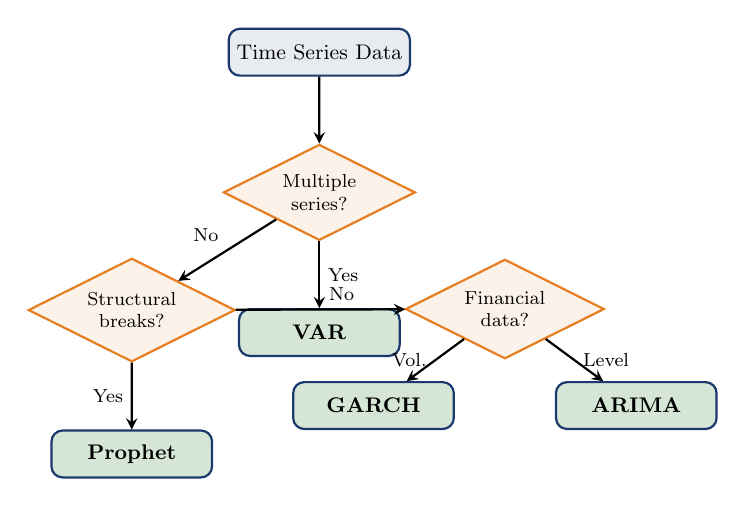
\begin{tikzpicture}[scale=0.85, transform shape,
        node distance=1.0cm,
        box/.style={rectangle, draw=MainBlue, thick, fill=MainBlue!10, rounded corners, minimum width=2.4cm, minimum height=0.7cm, align=center, font=\small},
        decision/.style={diamond, draw=Orange, thick, fill=Orange!10, aspect=2, align=center, font=\footnotesize},
        arrow/.style={->, thick, >=stealth}
    ]
        \node[box] (start) {Time Series Data};
        \node[decision, below=of start] (q1) {Multiple\\series?};
        \node[decision, below left=1.0cm and 1.3cm of q1] (q2) {Structural\\breaks?};
        \node[decision, below right=1.0cm and 1.3cm of q1] (q3) {Financial\\data?};
        \node[box, fill=Forest!20, below=of q1] (var) {\textbf{VAR}};
        \node[box, fill=Forest!20, below=of q2] (prophet) {\textbf{Prophet}};
        \node[box, fill=Forest!20, below left=0.7cm and 0cm of q3] (garch) {\textbf{GARCH}};
        \node[box, fill=Forest!20, below right=0.7cm and 0cm of q3] (arima) {\textbf{ARIMA}};
        \draw[arrow] (start) -- (q1);
        \draw[arrow] (q1) -- node[right] {\footnotesize Yes} (var);
        \draw[arrow] (q1) -- node[above left] {\footnotesize No} (q2);
        \draw[arrow] (q2) -- node[left] {\footnotesize Yes} (prophet);
        \draw[arrow] (q2) -- node[above right] {\footnotesize No} (q3);
        \draw[arrow] (q3) -- node[left] {\footnotesize Vol.} (garch);
        \draw[arrow] (q3) -- node[right] {\footnotesize Level} (arima);
    \end{tikzpicture}
    \end{center}
\end{frame}

\begin{frame}{Summary: Model Comparison}
    \begin{columns}[T]
        \column{0.55\textwidth}
        \begin{center}
        \footnotesize
        \begin{tabular}{llll}
            \toprule
            \textbf{Case} & \textbf{Challenge} & \textbf{Model} & \textbf{RMSE} \\
            \midrule
            Bitcoin & Volatility & GARCH & 2.15 \\
            Sunspots & Seasonality & Fourier & 31.10 \\
            Unemp & Break & SARIMA & 0.12 \\
            Economic & Multi-var & VAR & 1.53 \\
            \bottomrule
        \end{tabular}
        \end{center}

        \column{0.45\textwidth}
        \begin{center}
            \includegraphics[width=0.95\textwidth]{../charts/model_comparison.pdf}
        \end{center}
    \end{columns}

    \vspace{0.1cm}

    \begin{exampleblock}{Key Principle}
        \textbf{Match model to data characteristics}---no single model dominates.
    \end{exampleblock}
    \quantlet{TSA\_ch10\_model\_comparison}{https://github.com/QuantLet/TSA/tree/main/TSA_ch10/TSA_ch10_model_comparison}
\end{frame}

\begin{frame}{Comprehensive Model Comparison}
    \begin{center}
    \footnotesize
    \begin{tabular}{lcccc}
        \toprule
        \textbf{Feature} & \textbf{GARCH} & \textbf{Fourier} & \textbf{Prophet} & \textbf{VAR} \\
        \midrule
        \textbf{Target} & Volatility & Level & Level & Multiple \\
        \textbf{Seasonality} & No & Yes (long) & Yes (multi) & No \\
        \textbf{Structural breaks} & No & No & Yes & No \\
        \textbf{Multiple series} & No & No & No & Yes \\
        \textbf{Interpretable} & Medium & High & High & High \\
        \textbf{Parameters} & Few & $2K$ & Auto & Many \\
        \textbf{Missing data} & No & No & Yes & No \\
        \midrule
        \textbf{Best for} & Finance & Cycles & Business & Macro \\
        \bottomrule
    \end{tabular}
    \end{center}

    \vspace{0.3cm}

    \begin{columns}[T]
        \column{0.5\textwidth}
        \begin{block}{Our Results}
            \begin{itemize}
                \item GARCH: MAE=1.82 (volatility)
                \item Fourier: RMSE=31.10 (cycles)
                \item SARIMA: RMSE=0.12 (breaks)
                \item VAR: Avg RMSE=1.53 (multi)
            \end{itemize}
        \end{block}

        \column{0.5\textwidth}
        \begin{exampleblock}{Key Insight}
            Each model excels in its domain. The art is matching the model to the data characteristics.
        \end{exampleblock}
    \end{columns}
\end{frame}

\begin{frame}{Best Practices for Applied Forecasting}
    \begin{columns}[T]
        \column{0.5\textwidth}
        \begin{block}{Methodology}
            \begin{enumerate}
                \item \textbf{Explore} data
                \item \textbf{Test} stationarity
                \item \textbf{Split} train/val/test
                \item \textbf{Compare} on validation
                \item \textbf{Report} test metrics
            \end{enumerate}
        \end{block}

        \begin{alertblock}{Common Mistakes}
            \begin{itemize}
                \item Peeking at test data
                \item Over-fitting
                \item Ignoring assumptions
            \end{itemize}
        \end{alertblock}

        \column{0.5\textwidth}
        \begin{exampleblock}{Practical Tips}
            \begin{itemize}
                \item Start simple (naive)
                \item Add complexity if needed
                \item Check residuals
                \item Report CIs
            \end{itemize}
        \end{exampleblock}

        \begin{block}{Remember}
            ``All models are wrong, but some are useful.'' --- Box
        \end{block}
    \end{columns}
\end{frame}

%=============================================================================
% CONCLUSION
%=============================================================================
\begin{frame}{Key Takeaways}
    \begin{enumerate}
        \item \textbf{Rigorous Methodology}
        \begin{itemize}
            \item Train/validation/test split prevents overfitting
            \item Test set must remain untouched until final evaluation
        \end{itemize}

        \vspace{0.2cm}

        \item \textbf{Match Model to Data}
        \begin{itemize}
            \item Financial volatility $\rightarrow$ GARCH
            \item Long seasonality $\rightarrow$ Fourier terms
            \item Structural breaks $\rightarrow$ Prophet
            \item Multiple series $\rightarrow$ VAR
        \end{itemize}

        \vspace{0.2cm}

        \item \textbf{Interpret Results Carefully}
        \begin{itemize}
            \item Granger causality $\neq$ true causality
            \item Out-of-sample performance matters most
            \item Simpler models often work better
        \end{itemize}
    \end{enumerate}
\end{frame}

%=============================================================================
% REFERENCES
%=============================================================================
\begin{frame}{References}
    \footnotesize
    \begin{thebibliography}{99}
        \bibitem{box2015} Box, G.E.P., Jenkins, G.M., Reinsel, G.C., \& Ljung, G.M. (2015). \textit{Time Series Analysis: Forecasting and Control}. 5th ed., Wiley.

        \bibitem{hamilton1994} Hamilton, J.D. (1994). \textit{Time Series Analysis}. Princeton University Press.

        \bibitem{tsay2010} Tsay, R.S. (2010). \textit{Analysis of Financial Time Series}. 3rd ed., Wiley.

        \bibitem{hyndman2021} Hyndman, R.J., \& Athanasopoulos, G. (2021). \textit{Forecasting: Principles and Practice}. 3rd ed., OTexts.

        \bibitem{taylor2018} Taylor, S.J., \& Letham, B. (2018). Forecasting at Scale. \textit{The American Statistician}, 72(1), 37-45.

        \bibitem{bollerslev1986} Bollerslev, T. (1986). Generalized Autoregressive Conditional Heteroskedasticity. \textit{Journal of Econometrics}, 31(3), 307-327.

        \bibitem{sims1980} Sims, C.A. (1980). Macroeconomics and Reality. \textit{Econometrica}, 48(1), 1-48.
    \end{thebibliography}
\end{frame}

%=============================================================================
% DATA SOURCES
%=============================================================================
\begin{frame}{Data Sources}
    \begin{block}{Real Data Used in This Chapter}
        \begin{itemize}
            \item \textbf{Bitcoin}: Yahoo Finance (BTC-USD), 2019--2025
            \item \textbf{Sunspots}: Statsmodels Wolfer dataset, 1900--2008
            \item \textbf{US Unemployment}: Federal Reserve FRED (UNRATE), 2010--2025
            \item \textbf{Economic Variables}: FRED (GDPC1, UNRATE, CPIAUCSL, FEDFUNDS), 2000--2025
        \end{itemize}
    \end{block}

    \vspace{0.3cm}

    \begin{exampleblock}{Reproducibility}
        All analyses can be reproduced using the accompanying Jupyter notebook: \\
        \texttt{chapter10\_lecture\_notebook.ipynb}
    \end{exampleblock}
\end{frame}

%=============================================================================
% FINAL SLIDE
%=============================================================================
\begin{frame}[plain]
    \begin{tikzpicture}[remember picture, overlay]
        \fill[IDAred] (current page.north west) rectangle ([yshift=-0.15cm]current page.north east);
    \end{tikzpicture}

    \vfill
    \begin{center}
        {\Huge\textbf{\textcolor{MainBlue}{Thank You}}}\\[0.5cm]
        {\Large\textcolor{MediumGray}{Questions?}}\\[1cm]
        {\large Prof. Daniel Traian Pele, PhD}\\[0.2cm]
        {\texttt{danpele@ase.ro}}\\[0.5cm]
        {\footnotesize Bucharest University of Economic Studies}
    \end{center}
    \vfill

    \begin{tikzpicture}[remember picture, overlay]
        \fill[IDAred] (current page.south west) rectangle ([yshift=0.15cm]current page.south east);
    \end{tikzpicture}
\end{frame}

\end{document}
